\documentclass{article}
\usepackage[utf8]{inputenc}
\usepackage{float}
\usepackage{graphicx}
\usepackage{hyperref}
\usepackage{cleveref}
\usepackage{xcolor}
\usepackage{subcaption}
\hypersetup{
    colorlinks,
    linkcolor={black!50!black},
    citecolor={blue!50!black},
    urlcolor={blue!80!black}
}

\title{Visualizing fakenews as reported by euvsdisinfo.eu}
\author{Jesper Henrichsen \\{\small Supervised by: Pedro Ferreira}}
\begin{document}
\maketitle
\newpage
\tableofcontents
\newpage

%%%%
% Some title section: A visualization of fake news reported by euvsdisinfo.eu
%%%%
\section{Introduction}
Since the introduction of the internet, information has been able to reach further and faster than ever before. Recent developments of omnipresent social media has created the perfect platform for the spread of this information within the internet. For the sake of advertisement social media platforms has, since their introduction, only become better at targeting their audience with information that will capture their attention. As put by the team behind the newsfeed at Facebook: ``{\it The goal of News Feed is to deliver the right content to the right people at the right time (...)}''. However, a relevant question would be to whom it is implied to be {\it right} for.
\\ That it is not necessarily the user, has recently emerged as a likely answer.   
%However, the context is important to understand the consequence of this statement when the main purpose is to generate money through advertisement. Then, the statement comes to mean something alike whatever information will get the user to interact with the content, and in that equation, the quality of the actual content becomes irrelevant. 
% Then, the statement becomes something alike: the information that will get the user to interact with the content, and the equation becomes invariant to the quality of the information. 

Because of the nature of social media, it has proved an effective way to spread misinformation.
This report will describe the process of scraping and visualizing information from \href{http://euvsdisinfo.eu}{euvsdisinfo.eu}.
% \section{method}
\\\\
%%%%% ALTERNATE DRAFT:
% With most people using social media as their main source of information, targeted internet advertisement has proved to be the perfect storm for internet trolls, government agencies, and selfconcerned demagogues. The economist suggests that either humour or rage based posts are the most effective vessels for the spread of information on social media. The fact is, that most people will look to share content in a bid to make themselves appear to the world in a certain light.
% Echo chambers are created by the business model of social media firms, with clusters of other users that they are more similar with than with users in other clusters. The similarity measure is based on the likelihood of the users to interact with different types of content. The clusters are so finely tuned that one experiment don by researchers (?) showed that it was possible for anyone to infringe on any particular persons privacy and follow their geographical whereabouts via targeted ads for as little as \$1000 and a delay of only a couple of minutes. However, the clusters for targeted advertisement also optimizes the efficiency of information spread in terms of number of disposed users and the impact (?) as never before. This efficiency coupled with such information being misinformation, fake news, is possibly the greatest threat to democracy of our time. The fact that this tendency to use social media for spreading fake news exploits a conflict of interest for social media firms, for whom it is naive, and in some ways unfair, to expect them to be able to act as a governing body when one such interest is the core pillar of its business model - generate profit for shareholders. For a publiclly traded company, such interest always weighs the most, and any societal concerns will, if need be, come second (Noam Chomsky?). Therefore, in order to combat this great challenge for people to be able to discuss, debate, and reach compromises on the same empirical basis, there needs to be more regulation in this are, however new it may be. The fact taht so many individuals depends and uses social media as their main outlet makes it a concern not just for the individual, but for the society as a whole. Though, in order to make effective regulation, we need better understanding of a phenomena that in many regards are still new. \\\\

\section{Background}
Since 2015 the campaign \url{euvsdisinfo.eu}, has been run by the European External Action Service East Stratcom Task Force. The primary focus of the campaign is to identify and debunk pro-Kremlin disinformation. According to the 
The campaign enlists cases of debunked information from sources spanning from official news sites to twitter accounts, to non-online content such as interviews. The campaign included more than 3400 such cases that became part of the dataset this report is based on. The cases are all reported either by the campaign staff themselves, or one of the 400 collaborating organizations and individuals.
In \Cref{fig:cases} is seen how cases are listed on the website, the order of which is chronological with respect to the date it was reported.

\begin{figure}[H]
    \centering
    % \begin{subfigure}[b]{.3\textwidth}
    \caption{Example listing of disinformation cases on \url{euvsdisinfo.eu}}
    \label{fig:cases}
    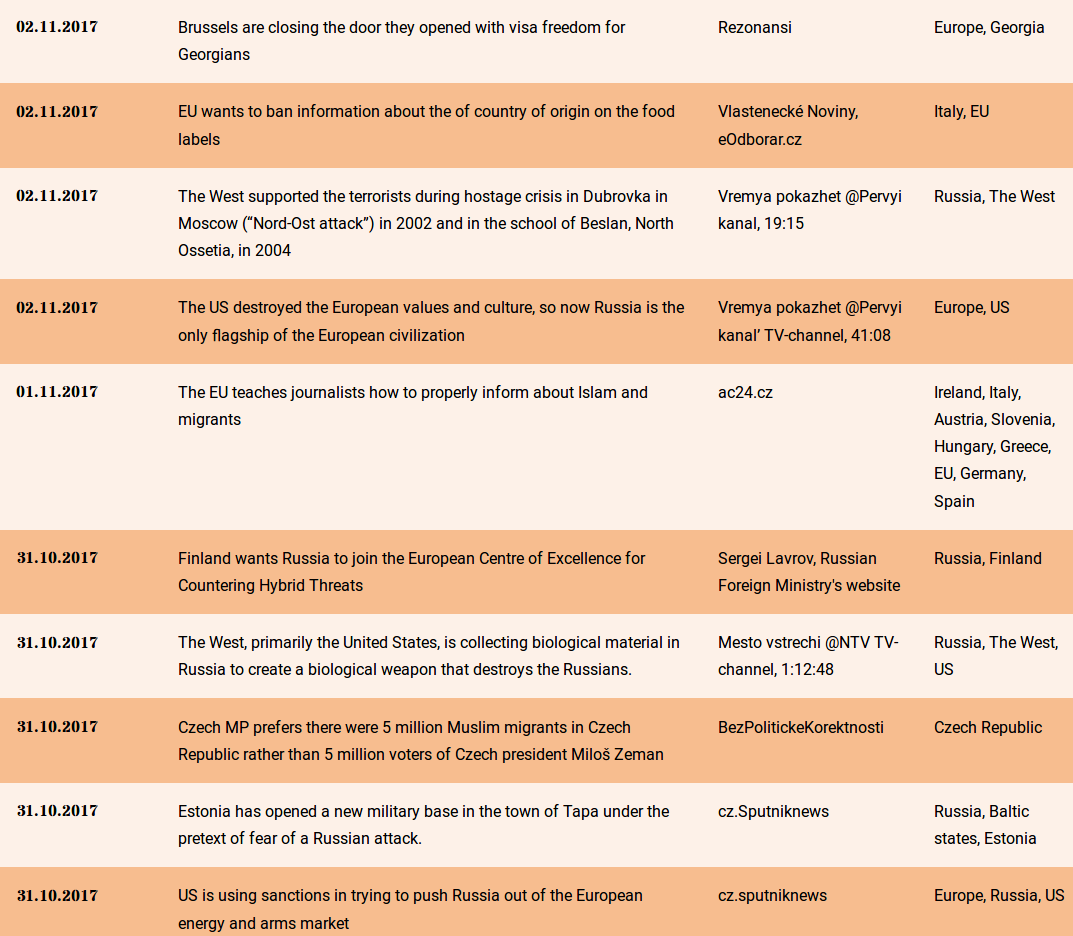
\includegraphics[width=.9\textwidth]{images/example_cases.png}
    % \end{subfigure}%
\end{figure}
\begin{figure}[H]
    % \begin{subfigure}[b]{.3\textwidth}
    \centering
    \caption{An example of the information for each case}
    \label{fig:single_case}
    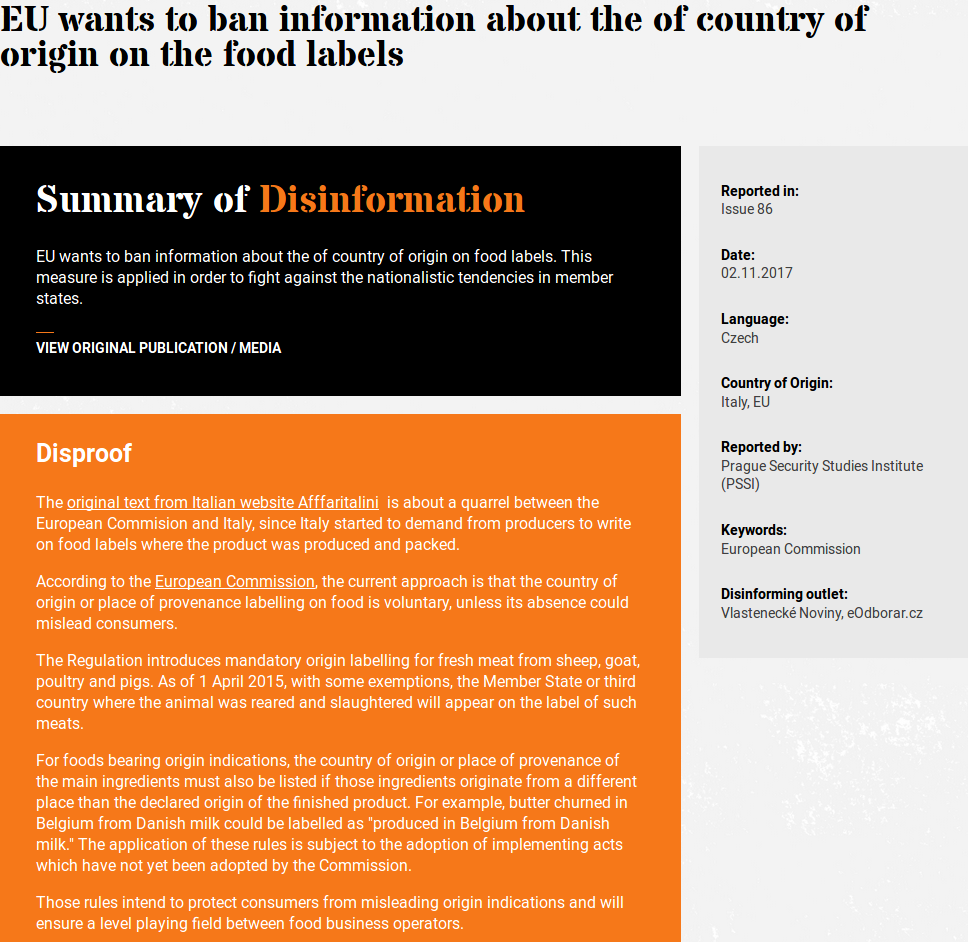
\includegraphics[width=.9\textwidth]{images/example_fakenews.png}
    % \end{subfigure}%
\end{figure}
\begin{figure}[H]
    % \begin{subfigure}[b]{.3\textwidth}
    \centering
    \caption{An example of a debunked news article from a Czech website}
    % \caption{An example of an original article from a Czech website that was debunked as  }
    \label{fig:fake_source}
    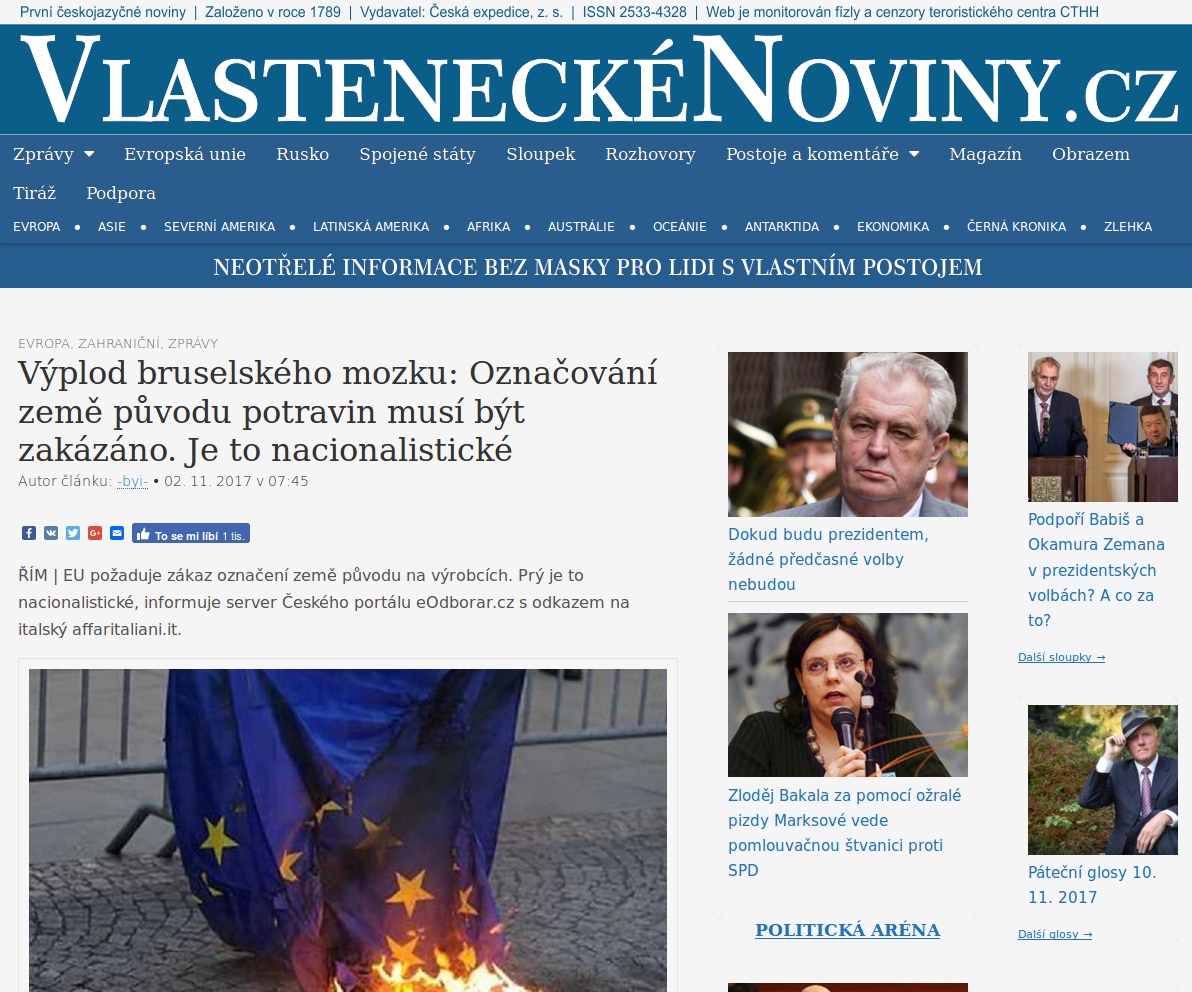
\includegraphics[width=.9\textwidth]{images/example_source.png}
    % \end{subfigure}
\end{figure}

\section{Acquiring information}
In this section, the approach to acquiring and extracting information for the visualization will be described.

\subsection{Article scraping and content extraction}
A general approach to extracting content is difficult because source of information can be any sort of media, whether digital or physical, in writing or a video. And because each website is different, then even building a scraper to extract the content of the subset that are online articles, will be difficult. Furthermore, in order to consider the names of locations that are being mentioned in the articles, the entire content is not necessary. For this reason I chose to use the meta tags to extract information about the content, summary, titles and descriptions. I would also filter on html tags such as the header tags, h1, h2, h3, h4, h5, h6 as well as the title tag used for setting the window title. I found through experiment that only considering the first found header tag worked best, the reason is that other header tags than the first one would often be titles of other news articles that the news site wants the user to click on.

The meta tag proved to be a very reliable way, since most news sites are interested in their content being shared, so its almost a must, in order to get content shared on social media.

In order to avoid duplicating content as much as possible I compared the content of a meta tag or html tag to the content that was already found in previous html tags. This approach resulted most often in a short paragraph of information about the article, including keywords, title and summary. Before applying the approach to the articles scraped from euvsdisinfo.eu, it was tested on sampled articles, such as danish news outlets. It was also tried on a sample of articles taken from the subreddits: r/politics, r/news, and r/worldnews, because these were good collections of all different news articles and news outlets. The results was used to evaluate qualitatively on the smaller sample. None of which turned out to have no content, and only one resulted in an extract only consisting of keywords. However, interestingly among the keywords were also the name of the country that the news story revolved around.
One thing that was clear from this however, was that locations were not always mentioned if the news revolved around well known state leaders such as Putin, Merkel or Trump. In such cases, only the names of the state leaders were present as indication of what countries were mentioned in the articles.

\subsection{Named entity recognition}
Named entity recognition is a research field within natural language processing concerned with recognizing names of things such as people, company names, or, as relevant for this project, locations. The study of recognizing location names within texts is one of the most studied ares of named entity recognition, however, still an ongoing research. A more in depth explanation of named entity recognition or even natural language processing, is however, beyond the scope of this project. Instead for the purposes of this project, I will rely on existing tools.

\subsection{Facebook}

\section{Results}

\section{Discussion}

\section{Conclusion}

\end{document}